

\section{wednesday}\index{Mednesday_lecture}
\subsection{Nonhomogenous equation}
\[L[y]=y^{\prime\prime}+p(t)y^\prime+q(t)y=g(t)\qquad\cdots(N)
\]
\[y^{\prime\prime}+p(t)y^\prime+q(t)y=0\qquad\cdots(H)\]
Suppose we have found total linearly independent solutions for the homogeneous equation $y_1$, $y_2$.
\[y=c_1y_1+c_2y_2
\]
Like we have done before, a resonable guess form of the nonhomogeneous solution may take the form of:
\[y_p=u_1(t)y_1+u_2(t)y_2
\]
\[y^\prime=u_1^\prime y_1+u_1y_1^\prime+u_2^\prime y_2+u_2y_2^\prime
\]
Furthermore, if we again compute $y^{\prime\prime}$, there will be  \emph{8} terms which will make things less interesting. Let's make $u_1^\prime y_1+u_2^\prime y_2=0$\\
\[
\begin{aligned}
y^{\prime\prime}&=u_1^\prime y_1\p&+u_1y_1\pp+u_2\p y_2\p&+u_2y_2\pp\\
py\p&=&pu_1y_1\p\qquad\quad&+pu_2y_2\p
\\
qy&=&qu_1y_1\qquad\quad&+qu_2y_2
\end{aligned}\]
Add them up together, we will get\\
$u_1\p y_1\p+u_2\p y_2\p=g$\\
Now, in order to get one solution, all we need to do is to solve;\\
$\left \{	\begin{gathered}
u_1\p y_1+u_2\p y_2=0\\
u_1\p y_1\p+u_2\p y_2\p=g.
\end{gathered}\right.$ \\
By cramer's rule (check MAT2040),
\[
u_1\p=\frac{\begin{vmatrix}0&y_2\\g&y_2\p\end{vmatrix}}{\begin{vmatrix}y_1&y_2\\y_1\p&y_2\p\end{vmatrix}}=-\frac{gy_2}{W[y_1,y_2]}
\]
In summary, we have find one particular solution $y_p$ for (N).\\
\\
Claim: any solution $z(t)$ for (N) must be of the form $z=y_p+c_1y_1+c_2y_2$ for some $c_1$, $c_2$.\\
\begin{proof}
For any given solution $z(t)$ for (N),\\
\[\begin{aligned}
(z-y_p)\pp+p(t)(z-y)\p+q(t)(z-y_p)&=z\pp+p(t)z\p+q(t)z-(y_p\pp+p(t)y_p\p+q(t)y_p)\\
&=q(t)-q(t)=0
\end{aligned}
\]
Therefore, $z-y_p$ is a solution of (H).
\end{proof}
However, as professor said,
\begin{figure}[H]
\centering
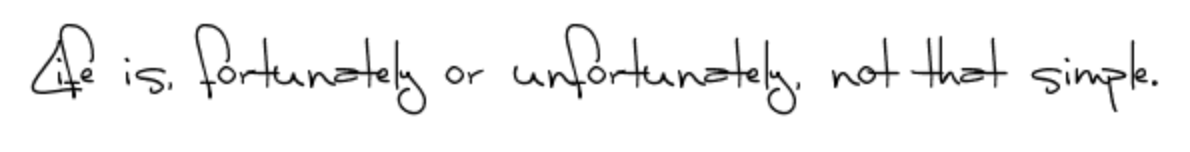
\includegraphics[width=12cm]{week6}
\end{figure}
Even a simplest nonhomogeneous equation can be a disaster to calculate.
\begin{example}
\[y\pp+y\p+y=t
\]
\[y\pp+y\p+y=0
\]
\[r\pp+r\p+1=0
\]
\[r=\frac{-1\pm\sqrt{1-4}}{2}=-\frac{1}{2}\pm\frac{\sqrt3}{2}i
\]
\[y_1=e^{-\frac{1}{2}t}\cos (\frac{\sqrt3}{2})\qquad y_2=e^{-\frac{1}{2}t}\sin (\frac{\sqrt3}{2})
\]
With the formula above and ``a little bit'' calculation,
\[u_1\p=\frac{-t^2e^{-\frac{1}{2}t}\sin(\frac{\sqrt{3}}{2}t)2e^{t}}{\sqrt3}
\]
\[u_1=\int t^2e^{\frac{1}{2}t}\sin(\frac{\sqrt3}{2}t)\diff t
\]
With similiar procedure, we can get $u_2$ which means $y_p$ is known which is the particular solution we want.\\
Anyway, you get the idea of how messy the computation can be.
\end{example}
\begin{remark}
It's much more easier to compute the solution of above example by reasonable guessing. See next section.


\end{remark}
\subsection{Undetermined coefficient question}
Sometimes, it's better to guess the form of the solution than calculating them in a formal way.
It's ok to have a reasonable guess.\\For example,
\[y\pp+y\p+y=t^2-t
\]
\[y_p=At^2+Bt+C
\]
\[y\p=2At+B
\]
\[y\pp=2A
\]
\[y\pp+y\p+y=2A+2At+B+At^2+Bt+C=At^2+(B+2A)t+2A+B+C
\]
\[A=1,\quad B=-2,\qquad C=0
\]
There are kinds of $g(t)$ that can use this method to solve. For instance, $t^ke^{at}$, $t^k\cos(wt)$, $t^k\sin(wt)$, $t6ke^{at}\cos(wt)$, \dots
\subsection{Mechanical Vibrations}
\begin{figure}[H]
\centering
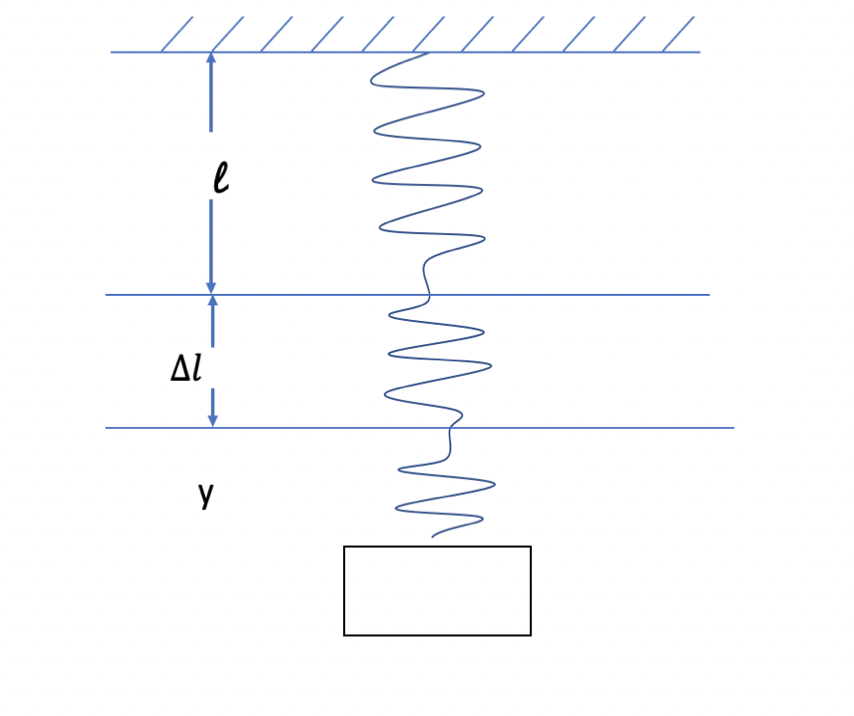
\includegraphics[width=10cm]{week6_M}
\end{figure}
The original length of spring is l. After placing block on it, it increase $\delta l$. With a force place on it, it, again, increase $y$.  $W$: be weight $m$g. $R$ is restoring force. $R=-(\Delta l+y)k$. Damping force $D=cy\p$. External force $F$
\[my\pp=mg-k(\Delta l+y)-cy\p+F
\]
\[mg=k\Delta l
\]
\[my\pp+cy\p+ky=F
\]
Let's see the case without damping force, i.e. $c=0$.
\[y\pp+\frac{k}{m}y=\frac{F}{M}
\]
\[y\pp+\frac{k}{m}y=\frac{F}{m}
\]
By physics, $w_0$ is the frequency.
\[w_0^2=\frac{k}{m}
\]
Free vibration($F=0$),
\[y\pp+w_0^2y=0
\]
\[r^2+w_0^2=0
\]
\[r=\pm iw_0
\]
\[\begin{aligned}y&=a\cos(w_0t)+b\sin(w_0t)\\
&=\sqrt{a^2+b^2}(\frac{a}{\sqrt{a^2+b^2}}\cos w_0t+\frac{b}{\sqrt{a^2+b^2}}\sin w_0t)\\
&=\sqrt{a^2+b^2}(\cos\delta\cos w_0t+\sin\delta\sin w_0t)\quad\text{Auxiliary angle method}\\
&=\sqrt{a^2+b^2}\cos(w_0t-\delta)
\end{aligned}
\]
\\
(2)Damped free vibration ($v\neq0$)
\[wy\pp+cy\p+ky=0
\]
\[mr^2+cr+k=0
\]
\[r=\frac{-c\pm\sqrt{c^2-4mk}}{2m}
\]



\begin{itemize}
\item
$c^2-4mk>0$:(over damped) 2 real roots both <0 $y=c_1e^{r_1t}+c_2e^{r_2t}\quad\rightarrow0$ not $\rightarrow\infty$
\item
$c^2-4mk<0$ 2 complex conjugate roots
\[r=-\frac{c}{2m}\pm i\frac{\sqrt{4mk-c^2}}{2m}
\]
\[\begin{aligned}y&=c_1e^{-\frac{c}{2m}t}\cos(\frac{\sqrt{4mk-c^2}}{2m}t)+c_2e^{-\frac{c}{2m}t}\sin(\frac{\sqrt{4mk-c^2}}{2m}t)\\
&=e^{-\frac{c}{2m}t}[c_1\cos(\frac{\sqrt{4mk-c^2}}{2m}t)+c_2\sin(\frac{\sqrt{4mk-c^2}}{2m}t)]\end{aligned}
\]
\item
$c^2=4mk\quad$ $c_1e^{-\frac{c}{2m}t}+c_2te^{-\frac{c}{2m}t}$
\end{itemize}
\begin{remark}
Those only hold when y is small.


\end{remark}







